   
\documentclass[11pt]{article}
\usepackage{amsmath,amsthm,verbatim,amssymb,amsfonts,amscd, graphicx}
\usepackage{graphicx}
\usepackage{listings}
\usepackage{float}
\usepackage{url}
\graphicspath{{./times/}}
\topmargin0.0cm
\headheight0.0cm
\headsep0.0cm
\oddsidemargin0.0cm
\textheight23.0cm
\textwidth16.5cm
\footskip1.0cm

\begin{document}
\title{CS 5220\\ Project 2 - Shallow Water Simulation}
\author{Marc Aurele Gilles (mtg79)\\ Sheroze Sheriffdeen(mss385)}
\maketitle

\section{Introduction}
Define structured grid computations \\
Define shallow water simulations \\
Math overview and associated abstractions in code\\

\section{Design Decisions}

The following sections describe the implementation changes from the original code found at \url{https://github.com/cornell-cs5220-f15/water}.

\subsection{Memory Layout}
The original solution a two dimensional vectors of 3-vectors to represent $U_t$, $F(U)_x$, and $G(U)_y$. During each time step, the solution accesses each element in the 2-D grid sequentially. Then, the \texttt{vector<vector<real>>} representation leads to memory accesses that are not local spatially. \\

Therefore, our solution chooses to use 3 separate two dimensional vectors per objects, $U_t$, $F(U)_x$, and $G(U)_y$. Thus, we are required in general to perform three loop iterations in place of a single loop in the original solution. But this approach leverages spatial locality, especially in \texttt{compute\_step} and \texttt{limited\_derivs} functions.

\subsection{Vectorization}

By observing the profiling information, we noticed that the original solution spends majority of its computational time in the functions \texttt{limited\_derivs}, \texttt{compute\_step} and \texttt{compute\_fg\_speeds}. By adopting the newer memory layout, we enabled spatially local memory accesses. We were also able to decompose \texttt{for} loops in the solution to improve vectorization. Refer to \texttt{ipo\_out\_vectorization.optrpt} in \url{https://github.com/sheroze1123/water/tree/vectorization} for more information. \\

In \texttt{compute\_fg\_speeds}, we performed two separate loops to compute flux and wave speeds. The flux computation and the wave speed computation for the complete grid is not handled by the \texttt{Physics} class. We used \texttt{\#pragma simd} directives to instruct the compiler the ability to vectorize these computations. The compiler was successfully able to vectorize these functions with an estimated potential speedup of 6.7. \\

\texttt{limited\_derivs} uses the \texttt{limdiff} function in \texttt{minmod.h}. To improve the vectorization of this computation, we changed the implementation of \texttt{limdiff} in the following ways. 

\begin{enumerate}
	\item \texttt{limdiff} now performs the computation on the complete grid instead of at one grid point.
	\item \texttt{limdiff} was decomposed as \texttt{limdiff\_x} and \texttt{limdiff\_y} to perform the limiter along the $x$ dimension and the $y$ dimension separately while still retaining unit stride. 
\end{enumerate}

\subsection{Parallelization}
The updated memory layout is amenable to parallelization via OpenMP, particular during the costly operations of \texttt{limited\_derivs} and \texttt{compute\_step}. \\

At the beginning of a call to \texttt{limited\_derivs} we initialize a team of threads using \texttt{\#pragma omp parallel}. Each application of the limiter to the components of $U_t$, $F(U)_x$, and $G(U)_y$ can be computed in parallel since we removed the data dependencies by creating 3 separate two dimensional arrays per component. We use the \texttt{\#pragma omp for} directive to parallelize the grid computation of each component. \\

In \texttt{compute\_step}, we initialize a team of threads using \texttt{\#pragma omp parallel}. The predictor step is now performed in parallel. Then, we create a barrier before proceeding to the corrector step since the the corrector step needs information from the predictor. After computing the corrector step, we perform a barrier before finally copying back to storage in parallel. The performance increase we observed via parallelization reached up to 3+ speedup. Results are plotted in section~\ref{sec:speedup}.


\subsection{Domain Decomposition}
\subsubsection{General Setup}
We decomposed the main grid into equally sized sub-grids, by first copying  each sub-grid into a separate array. Each sub-grid array contains its part of the main grid an outer layer of ghost cells which contain information about the neighboring cells or the cells on the opposite side of the main grid if the sub-domain is close to the boundary of the main grid as we use periodic boundary condition. We then perform some number of time steps on each independent sub-grid and finally synchronize by copying back the sub-grid (without the ghost cells) onto the main grid. 
\subsubsection{Ghost cells}

 The width of the layer of ghost cells for each sub-grid is 3t, where t is the number of time steps we wish to advance before synchronizing back onto the main grid. For each sub-grid, we declare a simulation object, and run the simulation essentially in the same manner as we would on the whole grid, except we never apply periodic boundary conditions on the sub-grids. Because of this, at each time step we perform without synchronization, we "loose" 3 layers of ghost cells, in the sense that the computation within this layer is erroneous. 
However, the rest of the grid is not contaminated with error, as information spreads through our simulation only by 3 layers per time step.

\subsubsection{Estimating the wave speed}
One of the big barrier to parallelizing this simulation is that we need to estimate the wave speed at each time step to be able to estimate a how big of a time step we can perform for the next iteration. Hence to allow each sub-grid to run from time t=0 to time t=tfinal, we would need know in advance the speeds at time t, t+dt1, t+(dt1+dt2)... $t+sum_{i=1}^{k-1}dti$ which we obviously don't have access to at time t. The problem is that we need to know at least a lower bound for all dt(j) as the number of time steps we will take to reach tfinal is directly proportional to the number of ghost cells we need to allocate for each sub-grid. Our solution is to estimate a lower bound for dtj as dtj = (1/k)*dt1 for all j, where k is some fixed constant (we have k=2 for example). Furthermore, for each sub grid at each time checks independently if the dtj is lower than (1/k)*dt1, our program throws an error and stops (but no synchronization to do this check). A better alternative, which we have not yet implemented would be to stop the computation if dtj is lower than k*dt1, double k and start the computation all over again from time t.


\section{Analysis}
\subsection{Profiling} \label{sec:prof}

The following time profiles were obtained on a 200x200 grid by advancing 100 frames. 

\subsubsection{Original solution}
We began the optimization by analyzing the time profiles of the original code. The following table shows the top 4 functions by CPU time. 
\lstinputlisting[basicstyle=\tiny]{./profiling/original.txt}

\subsubsection{Memory Layout Update}

\subsubsection{Vectorization}
Profiling of vectorization shows good improvements in performance, especially in the \texttt{limited\_derivs} and \texttt{compute\_fg\_speeds} functions, but a reduction in performance in the \texttt{compute\_step} function. The repetition of \texttt{limdiff\_x} and \texttt{limdiff\_y} is due to separation of components and axes in \texttt{limited\_derivs}. 
\lstinputlisting[basicstyle=\tiny]{./profiling/vectorization.txt}

\subsubsection{Parallelization}

\subsubsection{Domain Decomposition}


\subsection{Scaling Study} \label{sec:speedup}


\subsubsection{Strong Scaling Study}
Using a 500x500 grid and 100 frames, we observe the speedup with respect to the number of threads in our parallel implementation.

\begin{figure}[H]
    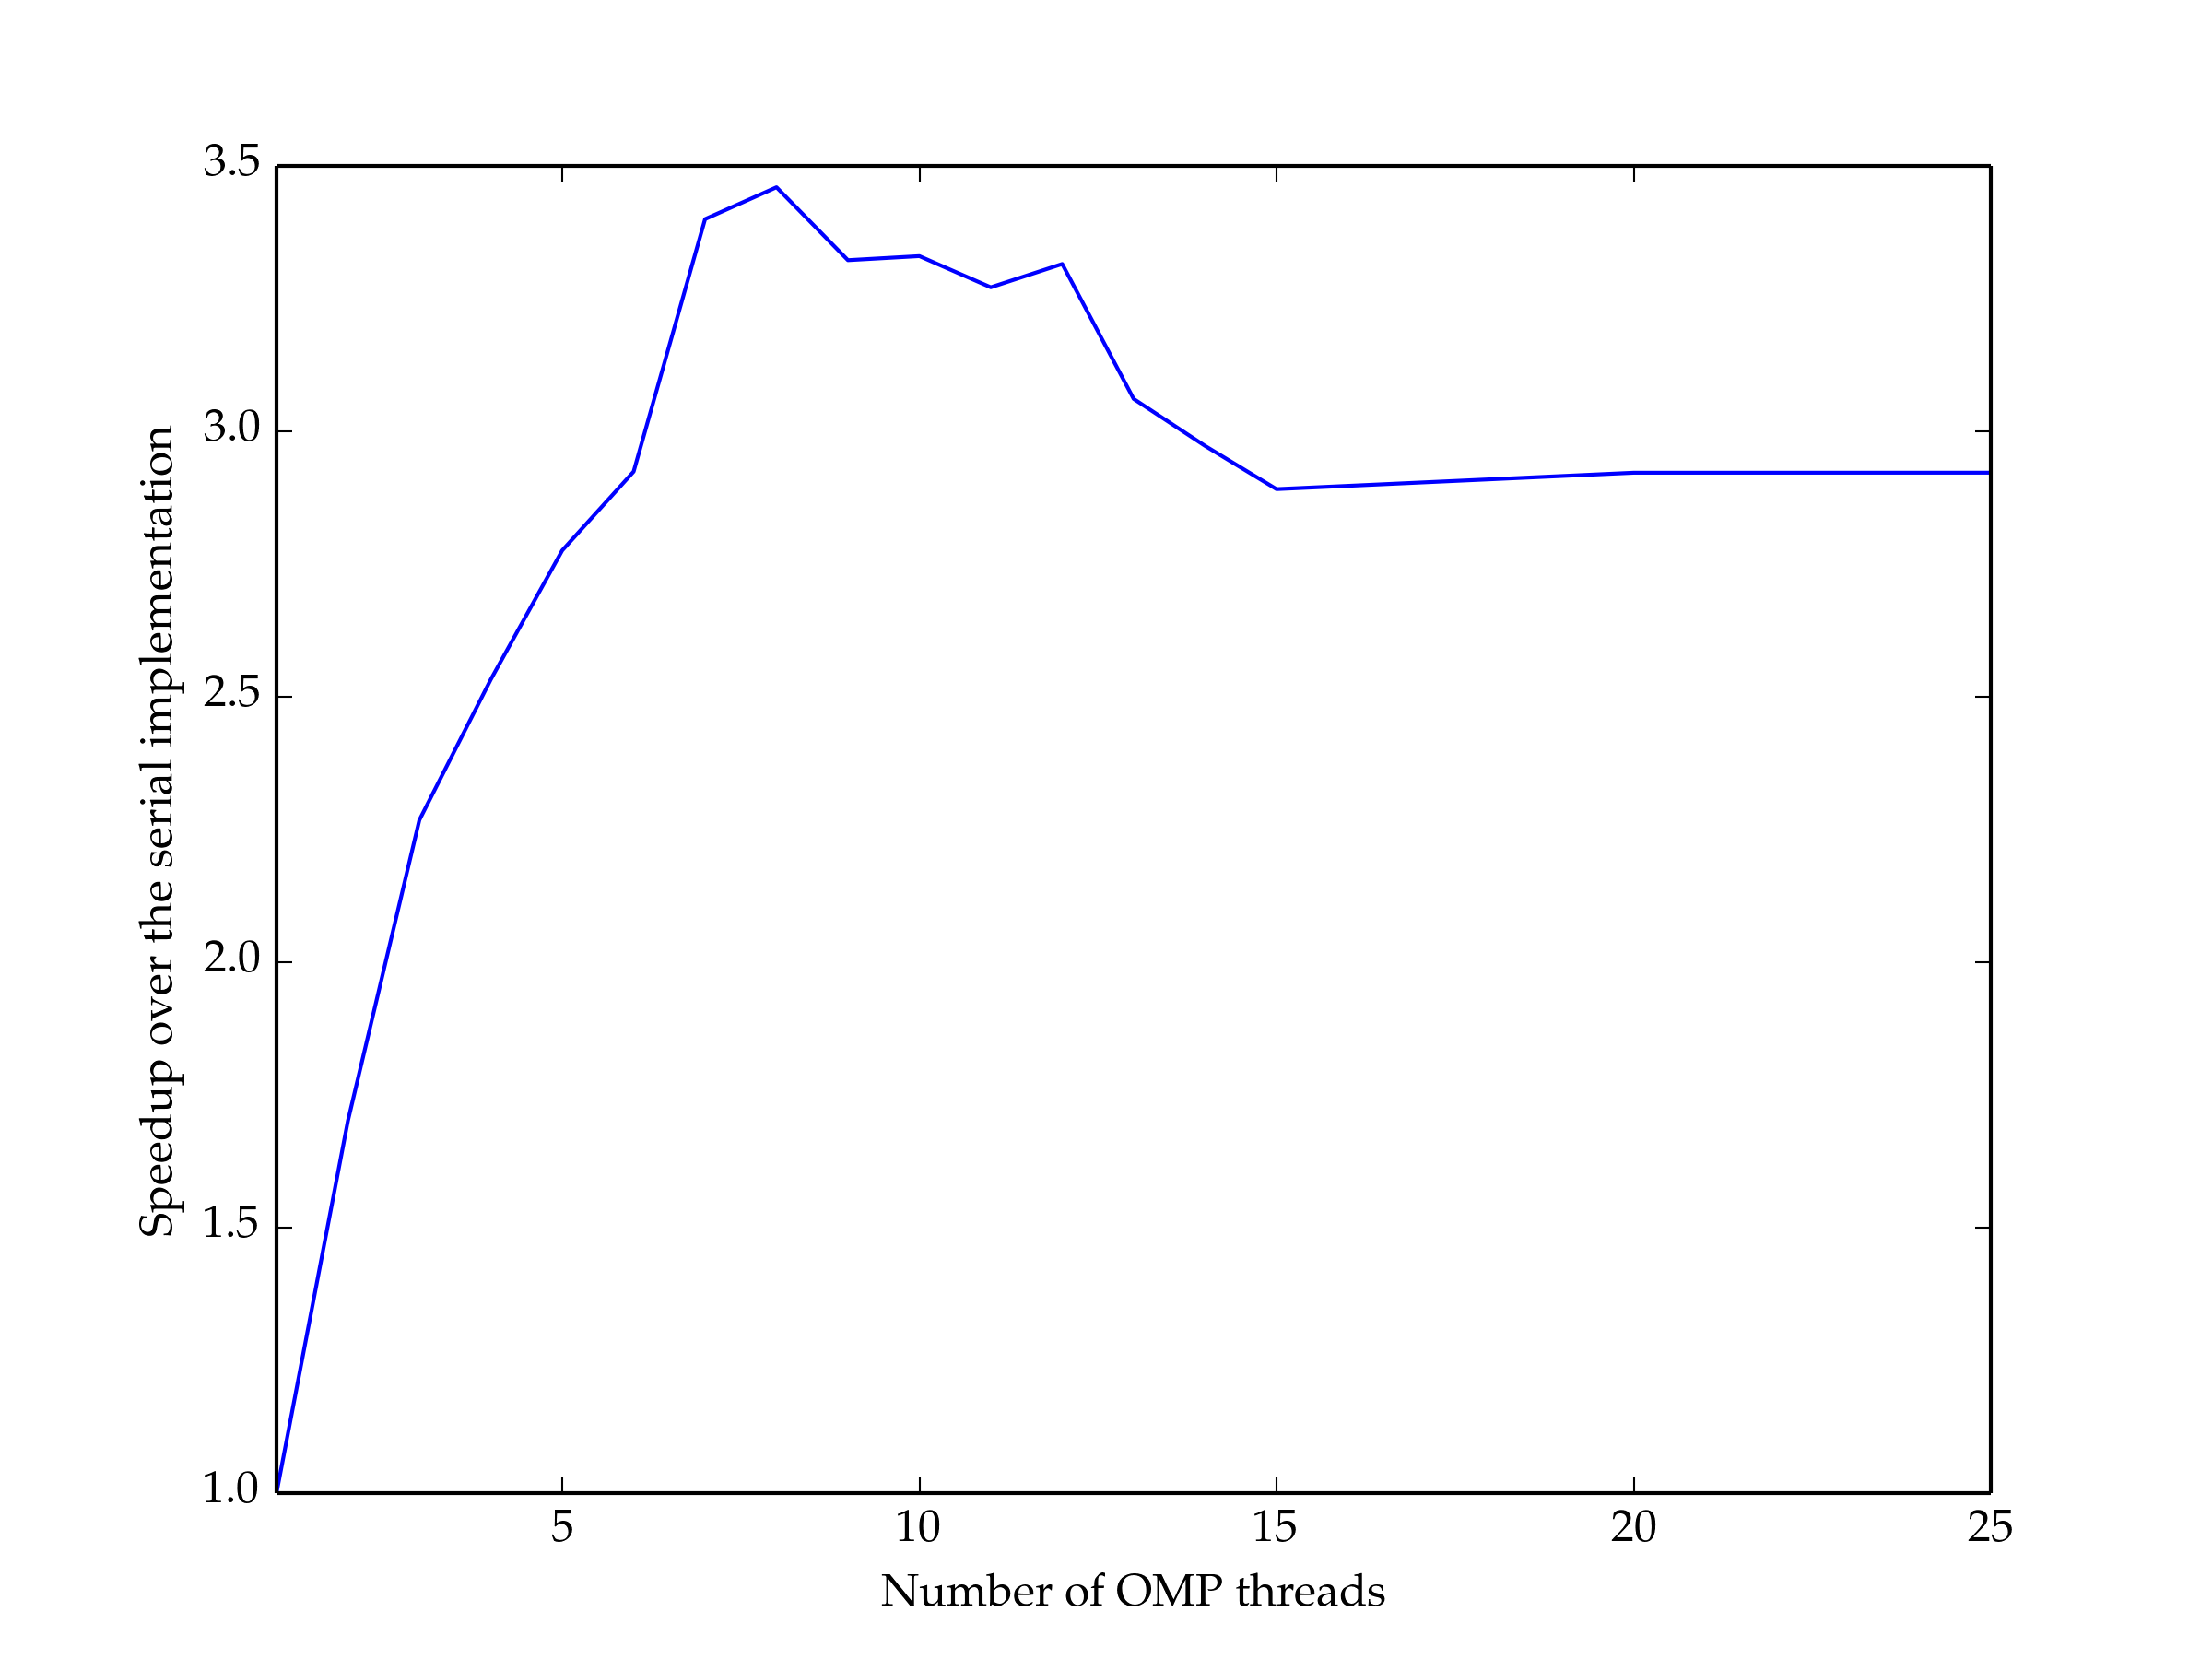
\includegraphics[width=0.9\textwidth]{./strong_scaling/strong_scaling.png}
    \caption{Speedup as a function of the number of threads}
    \label{fig:strong_scaling}
\end{figure} 


\subsubsection{Weak Scaling Study}

We vary the threads but keep the problem size/thread constant.
\begin{figure}[H]
    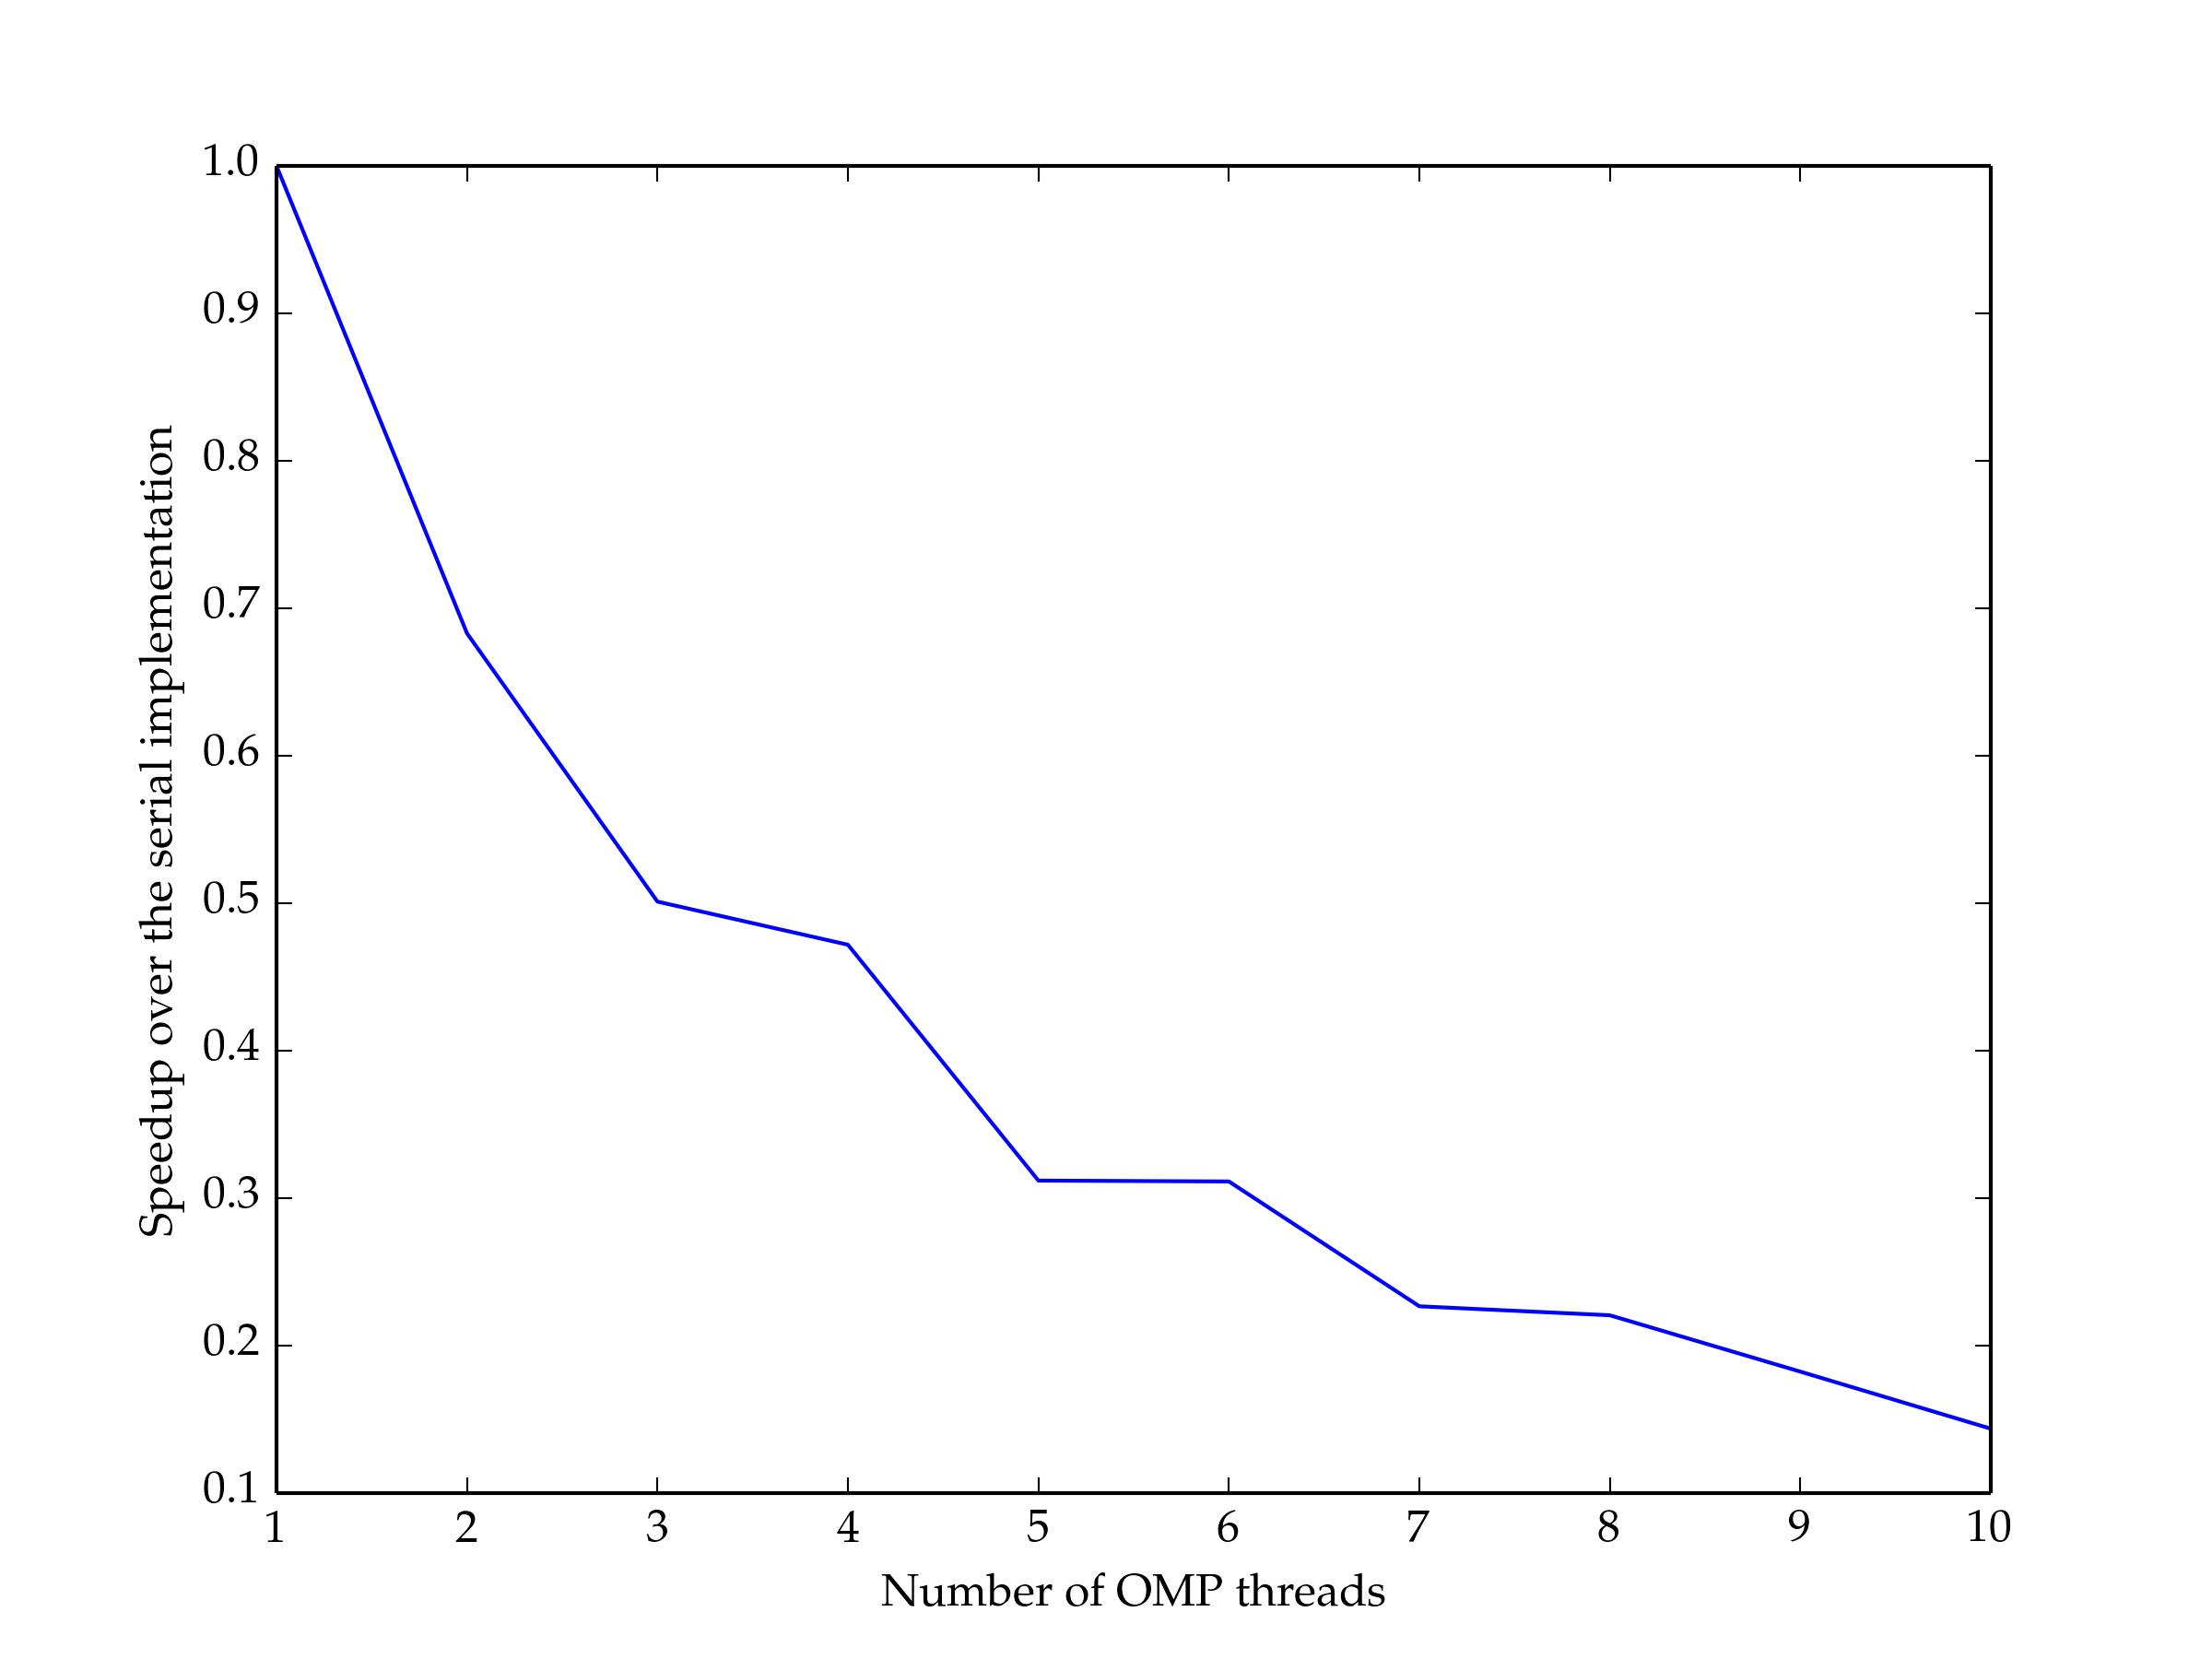
\includegraphics[width=0.9\textwidth]{./weak_scaling/weak_scaling.png}
    \caption{Speedup as a function of the number of threads}
    \label{fig:weak_scaling}
\end{figure} 



\begin{thebibliography}{9}
\bibitem{vectorization} 
Data Alignment to Assist Vectorization. (n.d.). Retrieved September 30, 2015, from \url{https://software.intel.com/en-us/articles/data-alignment-to-assist-vectorization}

\end{thebibliography}

 
 
\end{document}
